\section{Auswertung}
Die in der Auswertung bestimmten Ausgleichsrechnungen werden mit
dem Python Paket \emph{scipy.optimize}\cite{scipy} durchgeführt.
Des Weiteren werden die Fehler und insbesondere die Fehlerfortpflanzungen
mit dem Python Paket \emph{uncertainties}\cite{uncertainties} berechnet.

\subsection{Regressionsberechnung zur Bestimmung der Spannung im Verhältnis zum Abstand}\label{sec: ausgleich}

Für die verschiedenen Auswertungsteile wird immer eine Umrechnung von gemessenen Abständen
in die Spannung $U$ benötigt. Dazu wird an die Messwerte die in den Tabellen \ref{tab: spannung_abstand_zim}- \ref{tab: spannung_abstand_ioni} dargestellt sind,
eine Gerade der Form
\begin{equation}
  \label{eq: gerade}
  g(x)=mx+b
\end{equation}
berechnet.
Die sich daraus ergebenenen Regressionparameter sind in Tabelle \ref{tab: umrech} aufgelistet.
\FloatBarrier
\begin{table} 
\centering 
\caption{Aus Abbildung \ref{} abgelesene Spannung-Abstandspaare.} 
\label{tab: spannung_abstand_zim} 
\begin{tabular}{S S } 
\toprule  
{Abstand in $\si{\centi\meter}$} & {Spannung in $\si{\volt}$}  \\ 
\midrule  
 2.0  & 1.0\\ 
4.0  & 2.0\\ 
6.1  & 3.0\\ 
8.2  & 4.0\\ 
10.3  & 5.0\\ 
12.5  & 6.0\\ 
14.6  & 7.0\\ 
16.7  & 8.0\\ 
18.8  & 9.0\\ 
21.3  & 10.0\\ 
\bottomrule 
\end{tabular} 
\end{table}
\begin{table} 
\centering 
\caption{Aus Abbildung \ref{fig: messkurve_energie_hot} abgelesene Spannung-Abstandspaare.} 
\label{tab: spannung_abstand_hot} 
\begin{tabular}{S S } 
\toprule  
{Abstand in $\si{\centi\meter}$} & {Spannung in $\si{\volt}$}  \\ 
\midrule  
 1.9  & 1\\ 
4.1  & 2\\ 
6.1  & 3\\ 
8.3  & 4\\ 
10.2  & 5\\ 
12.3  & 6\\ 
14.5  & 7\\ 
16.7  & 8\\ 
18.8  & 9\\ 
20.9  & 10\\ 
\bottomrule 
\end{tabular} 
\end{table}
\begin{table} 
\centering 
\caption{Aus Abbildung \ref{fig: messkurve_frank_hertz} abgelesene Spannung-Abstandspare.} 
\label{tab: spannung_abstand_frank} 
\begin{tabular}{S S } 
\toprule  
{Abstand in $\si{\centi\meter}$} & {Spannung in $\si{\volt}$}  \\ 
\midrule  
 2.1  & 5\\ 
4.0  & 10\\ 
6.0  & 15\\ 
7.9  & 20\\ 
9.8  & 25\\ 
11.8  & 30\\ 
13.8  & 35\\ 
15.8  & 40\\ 
19.7  & 50\\ 
21.7  & 55\\ 
\bottomrule 
\end{tabular} 
\end{table}
\begin{table} 
\centering 
\caption{Aus Abbildung \ref{fig: messkurve_ioni} abgelesene Punkte, durch die eine Ausgleichgerade gelegt wird.} 
\label{tab: kodi_ioni} 
\begin{tabular}{S S } 
\toprule  
{Abstand in $\si{\centi\meter}$} & {Spannung in $\si{\volt}$}  \\ 
\midrule  
 1.3  & 2\\ 
2.7  & 4\\ 
4.2  & 6\\ 
5.4  & 8\\ 
6.8  & 10\\ 
8.0  & 12\\ 
9.4  & 14\\ 
10.5  & 16\\ 
12.0  & 18\\ 
13.5  & 20\\ 
14.5  & 22\\ 
15.8  & 24\\ 
17.2  & 26\\ 
18.5  & 28\\ 
\bottomrule 
\end{tabular} 
\end{table}
\begin{table} 
\centering 
\caption{Regressiongerade für die Abstand in Spannungs Umrechnung. Im Versuchsteil $1$ wird die Energieverteilung bei $T=\SI{28}{\celsius}$ untersucht, $2$ umfassst die Untersuchung der Energieverteilung bei $T=\SI{155}{\celsius}$, der dritte Abschnitt $(3)$ beschäftigt sich mit der Analyse der Frank-Hertz-Kurve und im Abschnitt $4$ wird die Ionisierungsspannung bestimmt.} 
\label{tab: umrech} 
\begin{tabular}{S S S S S } 
\toprule  
{Versuchsteil} & { $m$ in $\si{\volt\centi\meter\per}$} & {$\sigma_\mathrm{m}$ in $\si{\volt\centi\per\meter}$} & {$b$ in $\si{\volt}$} & {$\sigma_\mathrm{b}$ in $\si{\volt}$}  \\ 
\midrule  
 1  & 0.469  & 0.003  & 0.13  & 0.04\\ 
2  & 0.475  & 0.002  & 0.13  & 0.03\\ 
3  & 2.549  & 0.006  & -0.20  & 0.08\\ 
4  & 1.522  & 0.009  & -0.19  & 0.10\\ 
\bottomrule 
\end{tabular} 
\end{table}
Die Messwerte aus den Tabellen \ref{tab: spannung_abstand_zim}- \ref{tab: spannung_abstand_ioni} und die dazugehörigen Ausgleichsgeraden sind in
den Abbildungen \ref{fig: darstellung_1} und \ref{fig: darstellung_2} illustriert.
\begin{figure}
  \centering
  \begin{subfigure}{0.48\textwidth}
    \centering
    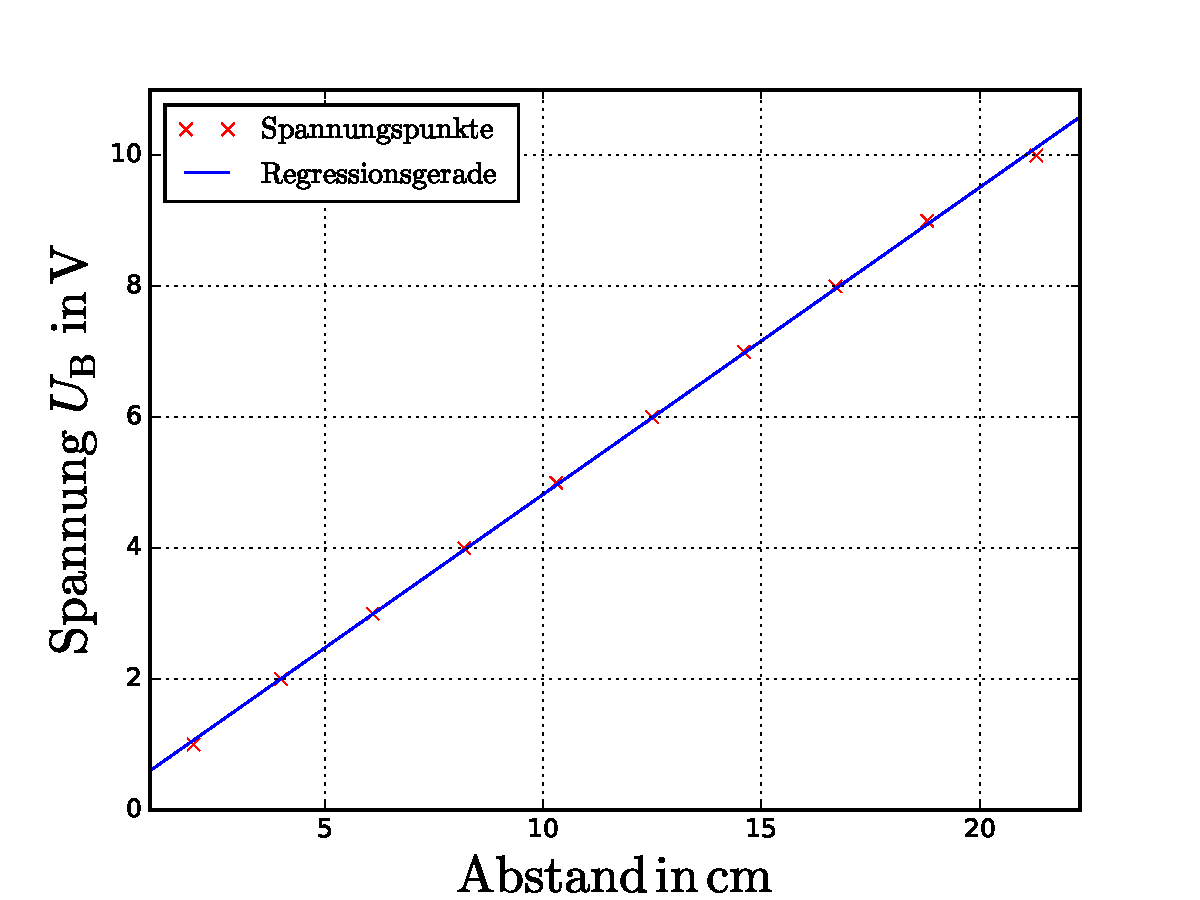
\includegraphics[width=1 \textwidth]{../Messdaten/zim.pdf}
    \caption{Graphische Darstellung des Ausgleichgraden für die Energieverteilung bei $\SI{28}{\degree}$.}
    \label{fig: energie_zim}
  \end{subfigure}
  \begin{subfigure}{0.48\textwidth}
    \centering
    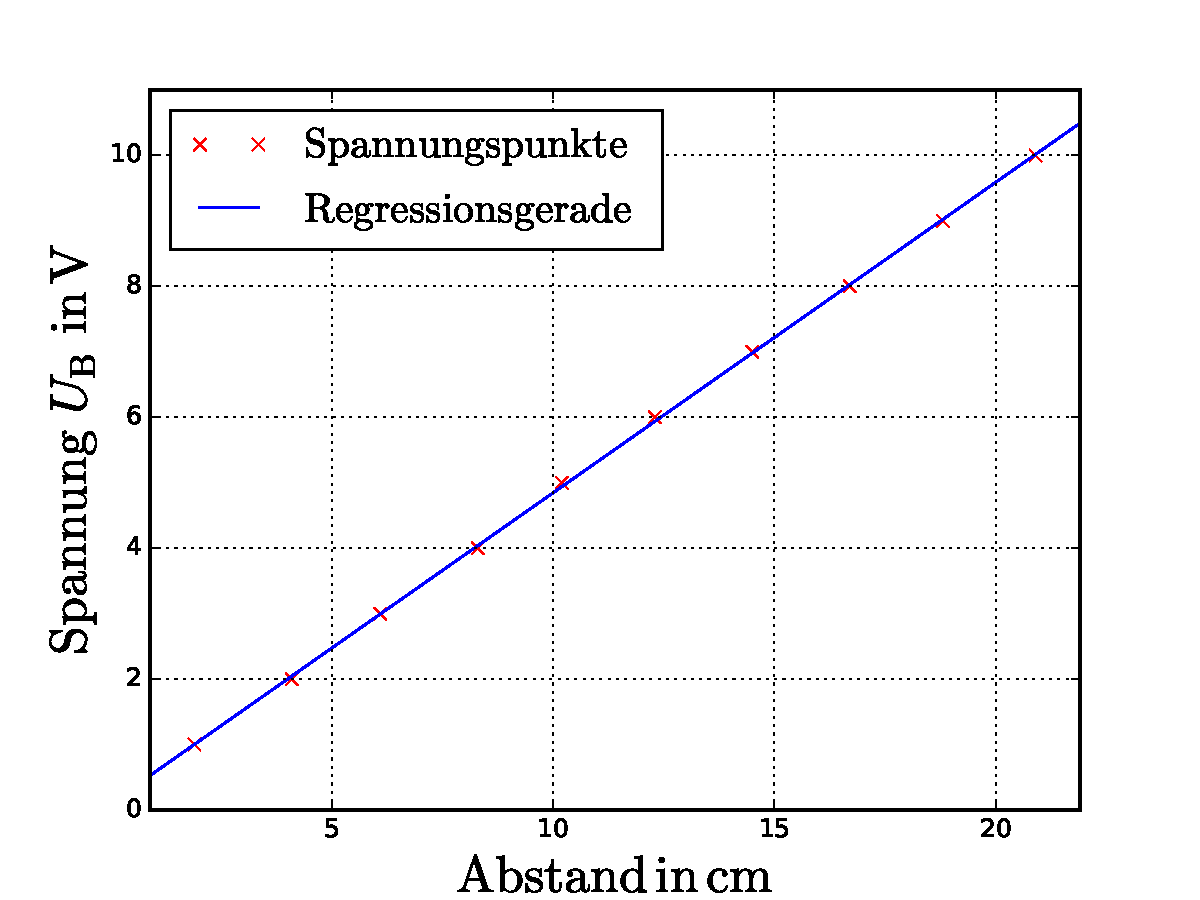
\includegraphics[width=1 \textwidth]{../Messdaten/spannungsfit_energieverteilung_150grad.pdf}
    \caption{Graphische Darstellung des Ausgleichgraden für die Energieverteilung bei $\SI{155}{\degree}$.}
    \label{fig: enrgie_hot}
  \end{subfigure}
  \caption{Darstellung der Ausgleichsgeraden für $(1)$ und $(2)$}
  \label{fig: darstellung_1}
\end{figure}
\begin{figure}
  \centering
  \begin{subfigure}{0.48\textwidth}
    \centering
    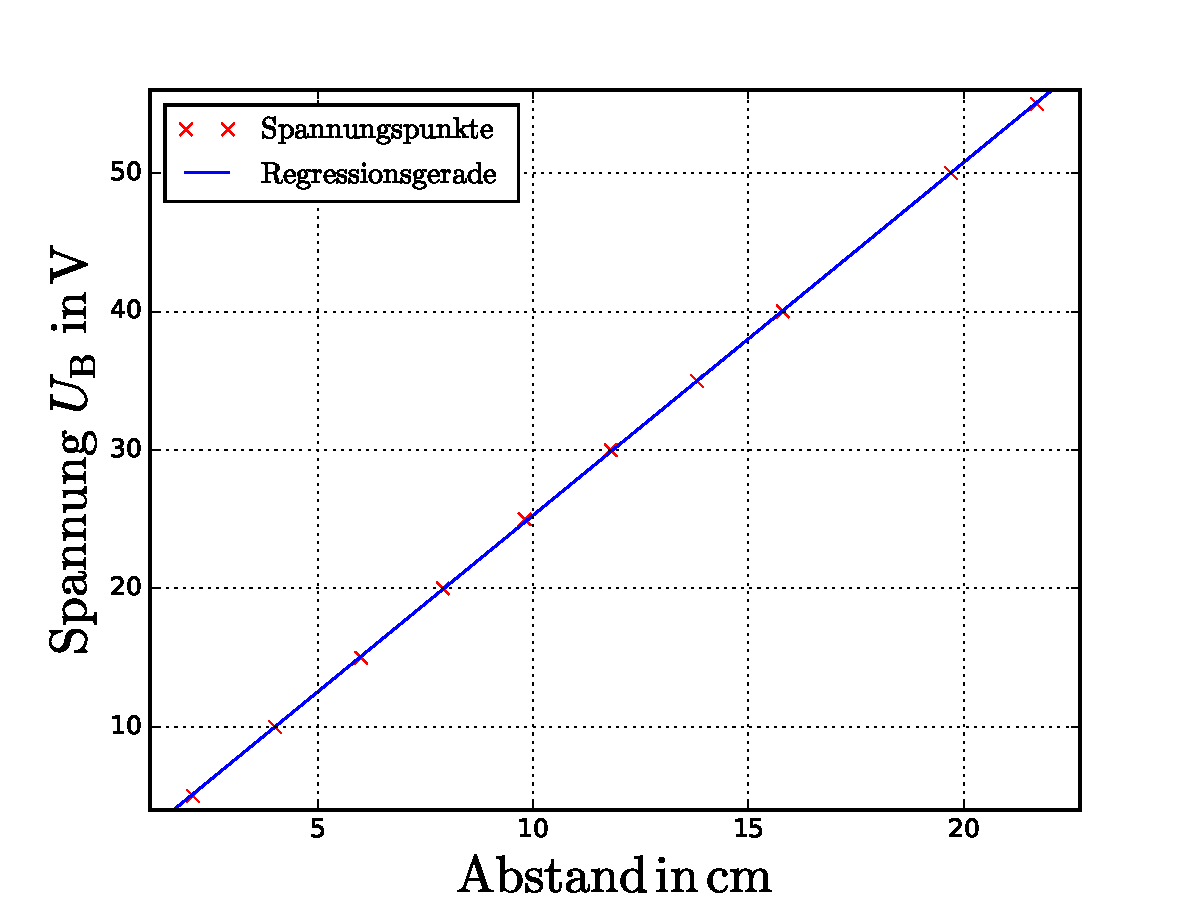
\includegraphics[width=1 \textwidth]{../Messdaten/frank_hertz_kuvre.pdf}
    \caption{Graphische Darstellung des Ausgleichgraden für Frank-Hertz-Kurve.}
    \label{fig: frank_hertz}
  \end{subfigure}
  \begin{subfigure}{0.48\textwidth}
    \centering
    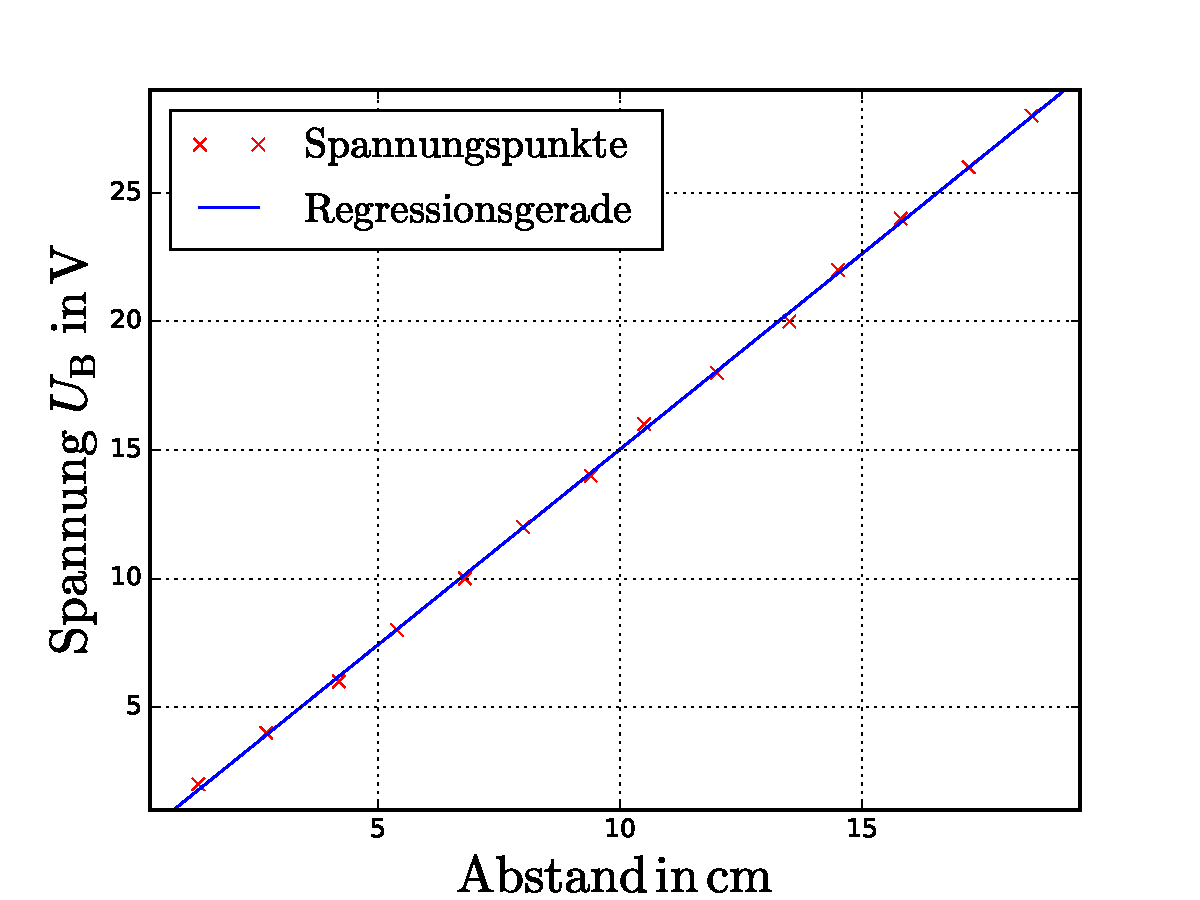
\includegraphics[width=1 \textwidth]{../Messdaten/ioni.pdf}
    \caption{Graphische Darstellung des Ausgleichgraden für die Untrersuchung der Ionisierungsspannung.}
    \label{fig: enrgie_hot}
  \end{subfigure}
  \caption{Darstellung der Ausgleichsgeraden für $(3)$ und $(4)$}
  \label{fig: darstellung_2}
\end{figure}
Die Fehler der Steigung und des y-Achsenabschnitt (vgl. \ref{tab: umrech}) werden
im Folgenden, auf Grund der geringen Größe im Vergleich zum eigentlichen Ablesefehler, nicht weiter betrachtet.
Somit erfolgt die Umrechnung von einem Abstand in eine Spannung
fehlerfrei.
\FloatBarrier

\subsection{Untersuchung der mittleren freien Weglänge}
\FloatBarrier
Wie in der Theorie erwähnt sollte die mittlere freie Weglänge $\ov{w}$ im Vergleich zum
Abstand $a$ zwischen Kathode und Beschleunigungselektode für Untersuchung der Frank-Hertz-Kurve (Abschnitt \ref{sec: frank})
etwa um den Faktor $1000-4000$ kleiner sein. Die freie Weglänge hängt über dem Druck mit der Temperatur zusammen.
Der Versuchsteil $1$ wurde bei einer Temperatur von $T=\SI{28}{\celsius}$ untersucht, $2$ bei $T=\SI{155}{\celsius}$,
$3$ bei $T=\SI{188}{\celsius}$ und $4$ bei $T=\SI{104}{\celsius}$ betrachtet (selbe Nummerierung wie in Tab. \ref{tab: umrech}).
Die Resultate sind in Tabelle \ref{tab: weg} zusammengefassst.
\begin{table} 
\centering 
\caption{Ergebnisse für die Verhältnisberechenung $a\/w$.} 
\label{tab: weg} 
\begin{tabular}{S S S S S } 
\toprule  
{$T$ in $\si{\celsius}$} & {$T$ in $\si{\kelvin}$} & {$p_{\mathrm{sät}} in $\si{\milli\bar}$} & {$\overline{w}$ in $\si{\centi\meter}$} & {$\frac{a/w}$}  \\ 
\midrule  
 28  & 301.15  & 0.007  & 0.4346  & 2\\ 
104  & 377.15  & 0.665  & 0.0044  & 229\\ 
150  & 423.15  & 4.822  & 0.0006  & 1663\\ 
188  & 461.15  & 18.399  & 0.0002  & 6344\\ 
\bottomrule 
\end{tabular} 
\end{table}

\subsection{Analyse der Energierverteilung bei $T=\SI{28}{\celsius}$}

Die aufgenommene Messkurve ist in Abbildung \ref{fig: messkurve_energie_zim} dargestellt.
\begin{figure}
  \centering
  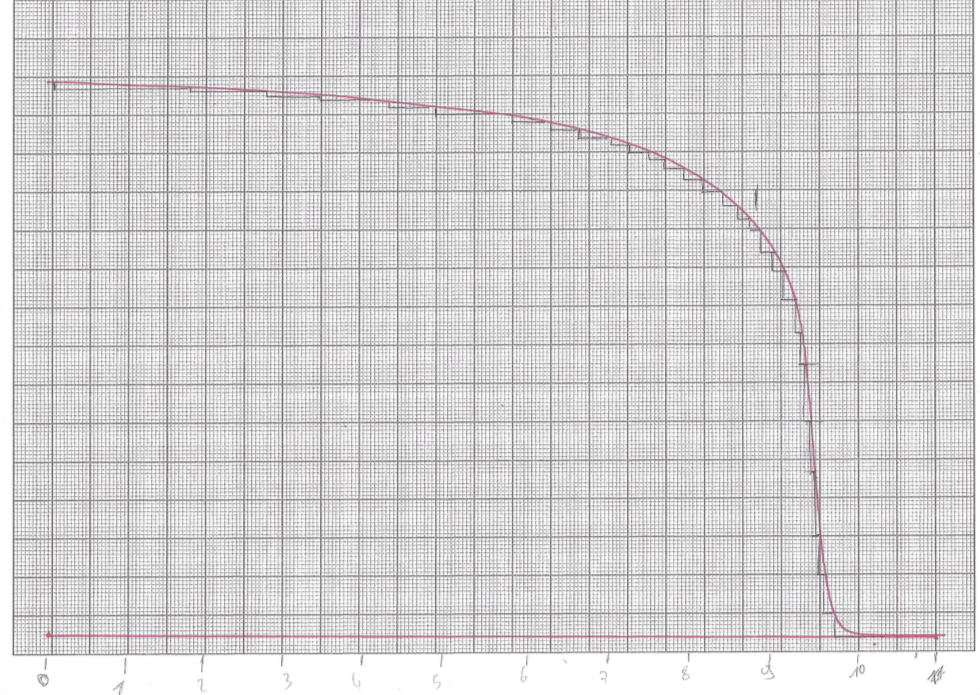
\includegraphics[width=0.8 \textwidth]{./pics/energieverteilung_zimmer.png}
  \caption{Aufgenommene Energieverteilung bei $T=\SI{28}{\celsius}$. Auf der $x$-Achse ist die Spannung $U\ua{a}$ in $\si{\volt}$ aufgetragen.
          Hingegen gibt die $y$-Achse die Stromstärke $I\ua{A}$ an. Zusätzlich sind in der Abbidung die für die Auswertugn entscheidenen Steigungsdreiecke zuer erkennen.}
  \label{fig: messkurve_energie_zim}
\end{figure}
Die in Abbildung \ref{fig: messkurve_energie_zim} Kurve gibt die Energieverteilung in \emph{integraler} Form an, durch anlegen von Steigugnsdreiecken der Form
\begin{equation}
  \label{eq:steigung}
    M=\frac{\Delta y}{\Delta x}=\frac{\Delta y}{x_2-x_1}
\end{equation}
kann die Kurve in ihre \emph{differntielle} Form transformiert werden.
Damit eine graphische Darstellung der differnetielle Kurve möglich ist, wird für jedes Koordiaaten Paar $(\Delta x,\Delta y)$ der Mittelpunkt
von $\Delta x$ als Messpunkt gesetzt. An diesem Messpunkt soll die Steigung $\frac{\Delta y}{\Delta x}$ genährt vorliegen.
Die Messpunkte werden mit den Ergebnissen aus Abschnitt \ref{sec: ausgleich} umgerechnet
Die aus dem Graph abgelsenen Werte sind in Tabelle \ref{tab: steigungen_zim} aufgelistet.
\begin{table} 
\centering 
\caption{Aus Abbildung \ref{fig: messkurve_energie_zim} abgelesene Steigungen.} 
\label{tab: steigungen_zim} 
\begin{tabular}{S S S S S S } 
\toprule  
{$x_1$ in $\si{\centi\meter}$} & {$x_2$ in $\si{\centi\meter}$} & { ${\Delta y}$ in $\si{\milli\meter}$} & {$\frac{\Delta y}{\Delta x}$ in \si{\milli\meter\per\centi\meter}} & {Messpunkt in $\si{\centi\meter}$} & {Messpunkt in $\si{\volt}$}  \\ 
\midrule  
 0.0  & 3.3  & 1.0  & 0.30  & 1.65  & 0.90\\ 
3.5  & 5.5  & 1.0  & 0.50  & 4.50  & 2.24\\ 
5.5  & 6.9  & 1.0  & 0.71  & 6.20  & 3.04\\ 
6.9  & 8.2  & 1.0  & 0.77  & 7.55  & 3.67\\ 
8.7  & 9.7  & 1.0  & 1.00  & 9.20  & 4.44\\ 
9.9  & 11.4  & 2.0  & 1.33  & 10.65  & 5.12\\ 
11.9  & 12.8  & 2.0  & 2.22  & 12.35  & 5.92\\ 
13.0  & 13.7  & 1.8  & 2.57  & 13.35  & 6.39\\ 
13.7  & 14.5  & 2.5  & 3.12  & 14.10  & 6.74\\ 
14.5  & 15.0  & 2.0  & 4.00  & 14.75  & 7.05\\ 
15.0  & 15.6  & 2.0  & 3.33  & 15.30  & 7.31\\ 
15.6  & 16.0  & 2.0  & 5.00  & 15.80  & 7.54\\ 
16.0  & 16.5  & 2.0  & 4.00  & 16.25  & 7.75\\ 
16.5  & 17.0  & 3.0  & 6.00  & 16.75  & 7.99\\ 
17.0  & 17.5  & 3.0  & 6.00  & 17.25  & 8.22\\ 
17.5  & 17.9  & 4.0  & 10.00  & 17.70  & 8.43\\ 
17.9  & 18.2  & 3.0  & 10.00  & 18.05  & 8.60\\ 
18.2  & 18.5  & 3.0  & 10.00  & 18.35  & 8.74\\ 
18.5  & 18.7  & 2.5  & 12.50  & 18.60  & 8.85\\ 
18.7  & 19.1  & 5.0  & 12.50  & 18.90  & 8.99\\ 
19.1  & 19.4  & 5.0  & 16.67  & 19.25  & 9.16\\ 
19.4  & 19.7  & 6.0  & 20.00  & 19.55  & 9.30\\ 
19.7  & 19.9  & 8.0  & 40.00  & 19.80  & 9.42\\ 
19.9  & 20.0  & 8.0  & 80.00  & 19.95  & 9.49\\ 
20.0  & 20.2  & 15.0  & 75.00  & 20.10  & 9.56\\ 
20.2  & 20.3  & 13.0  & 130.00  & 20.25  & 9.63\\ 
20.3  & 20.4  & 16.0  & 160.00  & 20.35  & 9.67\\ 
20.4  & 20.5  & 10.0  & 100.00  & 20.45  & 9.72\\ 
20.6  & 20.9  & 10.0  & 33.33  & 20.75  & 9.86\\ 
20.9  & 22.0  & 5.0  & 4.55  & 21.45  & 10.19\\ 
\bottomrule 
\end{tabular} 
\end{table}
Die Darstellung der differntiellen Kurve ist in Abb. \ref{fig: energie_zim_diff} zu finden.
\begin{figure}
  \centering
  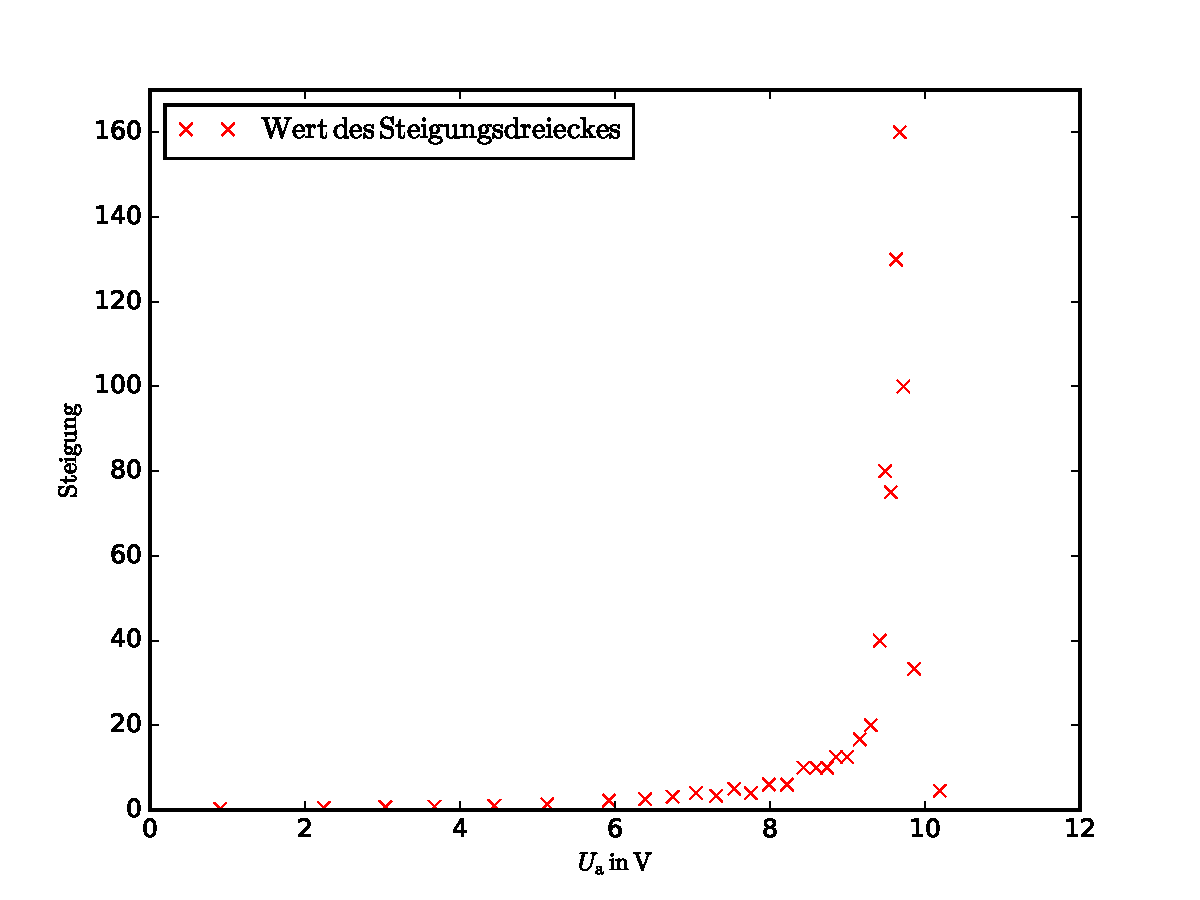
\includegraphics[width=0.8 \textwidth]{../Messdaten/energie_zim.pdf}
  \caption{Die Energiervertielung bei $T=\SI{28}{\celsius}$ in differentieller Form.}
  \label{fig: energie_zim_diff}
\end{figure}
Das Maximum der Abbildung liegt bei $U\ua{max}=\SI{9.67}{\volt}$. Zum Zeipunkt der Messung
lag eine Beschleunigungsspannung $U\ua{b}=\SI{11}{\volt}$ an.
Das Kontaktpotential $K$ kannn somit bestimmt werden:
\begin{equation}
\label{eq:k_energie_zim}
  K\ua{en}=U\ua{B}-U\ua{max}=\SI{1.33}{\volt}
\end{equation}
\FloatBarrier
\subsection{Analyse der Energierverteilung bei $T=\SI{150}{\celsius}$}
\FloatBarrier
Die aus dem Experiment resultierende Messkurve ist in Abbildung \ref{fig: messkurve_energie_hot} dargestellt.
\begin{figure}
  \centering
  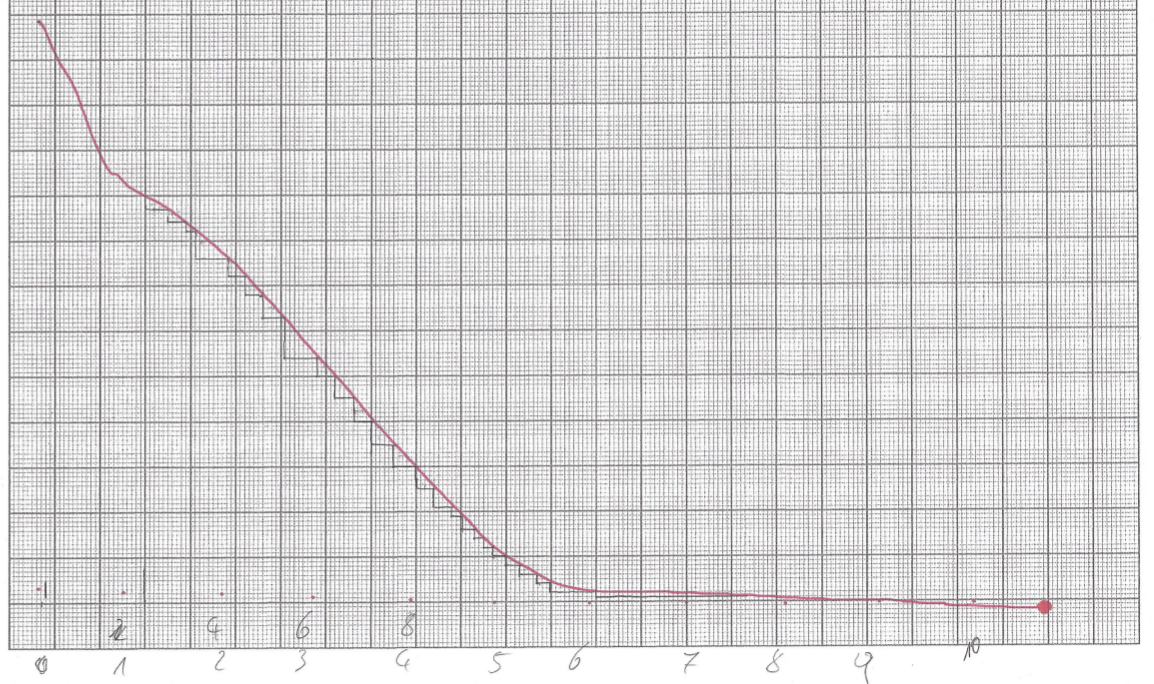
\includegraphics[width=0.8 \textwidth]{./pics/energieverteilung_hot.png}
  \caption{Aufgenommene Energieverteilung bei $T=\SI{150}{\celsius}$. Auf der $x$-Achse ist die Spannung $U\ua{a}$ in $\si{\volt}$ aufgetragen.
          Hingegen gibt die $y$-Achse die Stromstärke $I\ua{A}$ an. Zusätzlich sind in der Abbidung die für die Auswertugn entscheidenen Steigungsdreiecke zuer erkennen.}
  \label{fig: messkurve_energie_hot}
\end{figure}
Um die Kurve in die differntiele Form zu transformieren, wird wie im vorherigen Kaptiel vorgegangen.
Die Steigungen wurden mit Formel \eqref{eq:steigung} berechnet und sind in Tabelle \ref{tab: steigungen_hot} notiert.
\begin{table} 
\centering 
\caption{Aus Abbildung \ref{fig: messkurve_energie_hot} abgelesene Steigungen.} 
\label{tab: steigungen_hot} 
\begin{tabular}{S S S S S } 
\toprule  
{$x_1$ in $\si{\centi\meter}$} & {$x_2$ in $\si{\centi\meter}$} & { ${\Delta y}$ in $\si{\milli\meter}$} & {$\frac{\Delta y}{\Delta x}$ in \si{\milli\meter\per\centi\meter}} &{$x_1$ in $\si{\volt}$}  \\ 
\midrule  
 2.4  & 2.9  & 3.0  & 6.00  & 1.24\\ 
2.9  & 3.3  & 3.0  & 7.50  & 1.48\\ 
3.3  & 3.5  & 2.0  & 10.00  & 1.67\\ 
3.5  & 3.8  & 2.0  & 6.67  & 1.76\\ 
3.8  & 4.5  & 6.0  & 8.57  & 1.90\\ 
4.5  & 4.9  & 4.0  & 10.00  & 2.23\\ 
4.9  & 5.3  & 4.0  & 10.00  & 2.42\\ 
5.3  & 5.8  & 5.0  & 10.00  & 2.61\\ 
5.8  & 6.5  & 9.0  & 12.86  & 2.85\\ 
6.5  & 6.9  & 4.0  & 10.00  & 3.18\\ 
6.9  & 7.3  & 5.0  & 12.50  & 3.37\\ 
7.3  & 7.8  & 5.0  & 10.00  & 3.56\\ 
7.8  & 8.2  & 5.0  & 12.50  & 3.80\\ 
8.2  & 8.6  & 4.0  & 10.00  & 3.99\\ 
8.6  & 9.0  & 4.0  & 10.00  & 4.18\\ 
9.0  & 9.2  & 2.0  & 10.00  & 4.37\\ 
9.2  & 9.5  & 3.0  & 10.00  & 4.47\\ 
9.5  & 9.7  & 2.0  & 10.00  & 4.61\\ 
9.7  & 9.9  & 2.0  & 10.00  & 4.70\\ 
9.9  & 10.2  & 2.0  & 6.67  & 4.80\\ 
10.2  & 10.5  & 2.0  & 6.67  & 4.94\\ 
10.5  & 10.9  & 2.0  & 5.00  & 5.08\\ 
10.9  & 11.2  & 2.0  & 6.67  & 5.27\\ 
11.2  & 12.2  & 2.0  & 2.00  & 5.41\\ 
12.2  & 16.2  & 2.0  & 0.50  & 5.89\\ 
\bottomrule 
\end{tabular} 
\end{table}
Die Spannungen wurden wieder mit den Resultaten aus Kapitel \ref{sec: ausgleich} errechnet.
Eine Illustration der differentiellen Kurve ist in Abbildung \ref{fig: energie_hot_diff} präsentiert
\begin{figure}
  \centering
  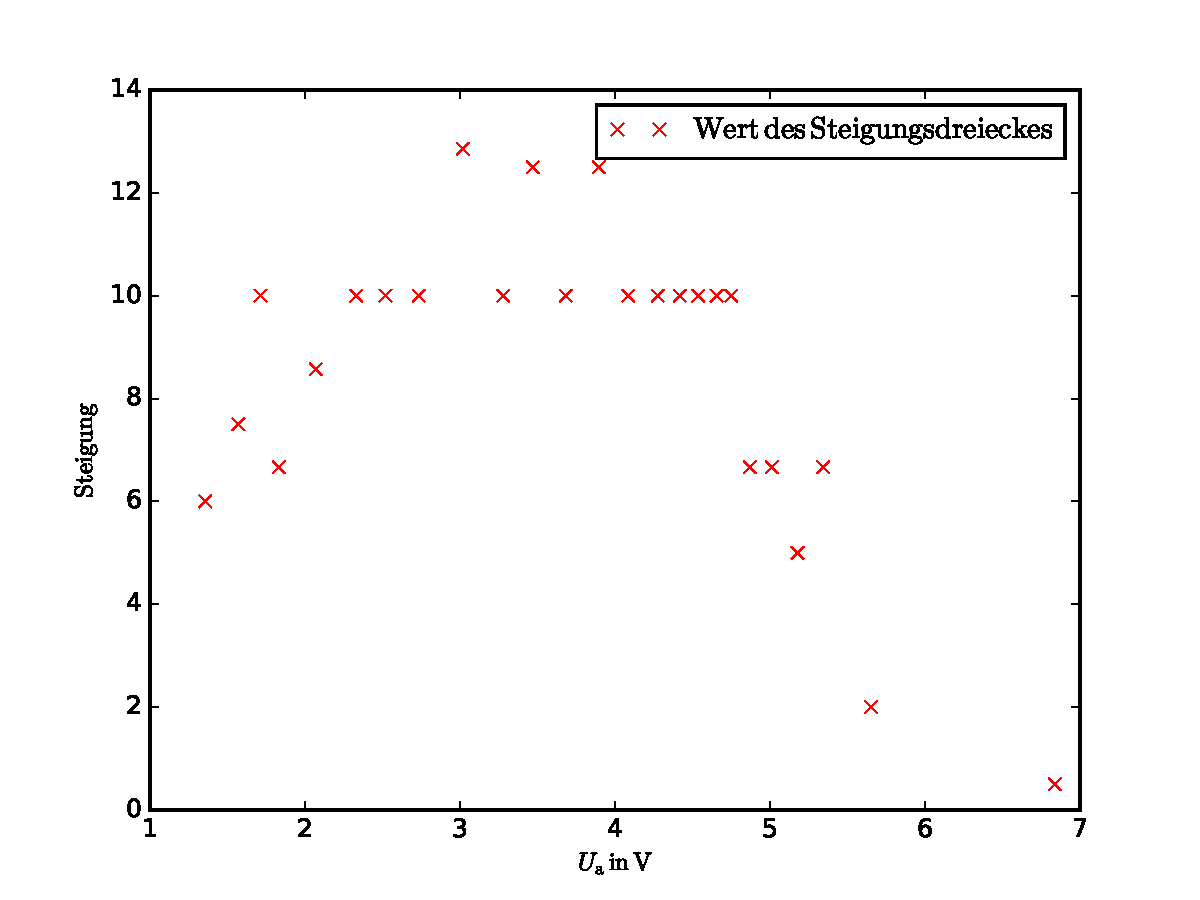
\includegraphics[width=0.9 \textwidth]{../Messdaten/energie_hot.pdf}
  \caption{Die Energiervertielung bei $T=\SI{150}{\celsius}$ in differentieller Form.}
  \label{fig: energie_hot_diff}
\end{figure}
Wie in Abbildung \ref{fig: messkurve_energie_hot} zu erkennen, beginnen die Steigungsdreiecke erst ab
einer Spannung von $U\ua{anf}=\SI{1.24}{\volt}$, dies ist damit zu Begründen das für Spannungen $U<U\ua{ua}$
der Kurvenverlauf keinen physikallischen Zusammenhang beschreibt.
Zusätzlich lässt sich in der differentiellen Kurve kein klares Maximum ausmachen, die dazugehörige Ursache wird in
der Diskussion besprochen.

Abschließend ist noch der signifikante Unterschied zwischen den Graphen \ref{fig: messkurve_energie_hot} und \ref{fig: messkurve_energie_zim}
zu erläutern. Beim betrachten der Tabelle \ref{tab: weg} fällt auf das sich die Werte für $\frac{a}{w}$ um den Faktor $\approx 800$ unterscheiden.
Das bedeutet dass die ausgelösten Elektron beim Messvorgang von \ref{fig: messkurve_energie_hot} deutlich öfters mit den
Quecksilberatome gewechselt wirkt haben. Auf Grund besitzen die Elektron nach dem Stoß nicht mehr genügend
Energie, um den wachsenden Gegenfeld $U\ua{A}$ zu durchqueren. Damit ist das schnelle konvergieren der Kurve zu erklären.
Eine Aussage über die Energieverteilung der Elektronen ist somit nicht möglich.
\FloatBarrier
\subsection{Untersuhung der Frank-Hertz-Kurve}\label{sec: frank}
\FloatBarrier
Die vom X-Y Schreiber aufgezeichnete Frank-Hertz-Kurve ist in der Illustration \ref{fig: messkurve_frank_hertz} abgebildet.
\begin{figure}
  \centering
  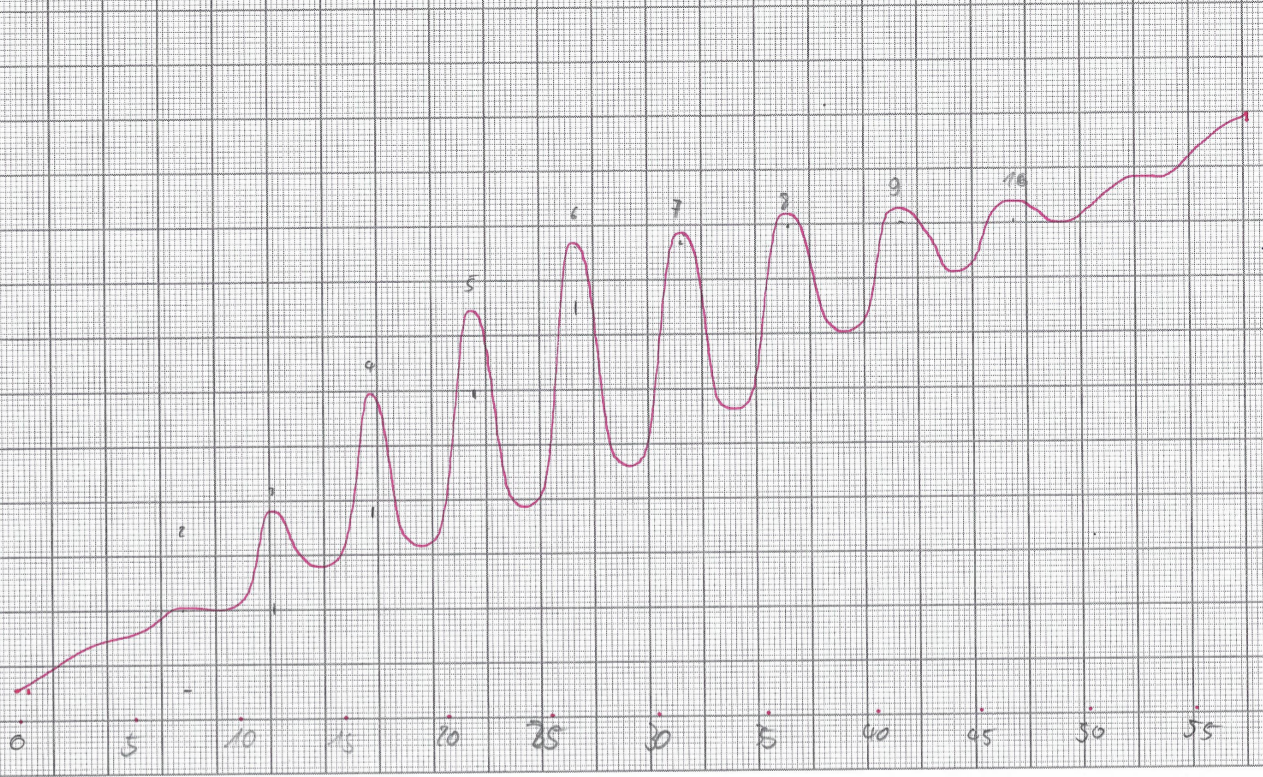
\includegraphics[width=0.8 \textwidth]{./pics/frank_hertz_kurve.png}
  \caption{Aufgenommene Frank-Hertz-Kurve bei $T=\SI{188}{\celsius}$. Auf der $x$-Achse ist die Spannung $U\ua{B}$ in $\si{\volt}$ aufgetragen.
          Hingegen gibt die $y$-Achse die Stromstärke $I\ua{A}$ an. Zusätzlich sind die erkennbaren Maxima nummeriert.}
  \label{fig: messkurve_frank_hertz}
\end{figure}
Die aus der Abbbildung abgelesenen Abstände der Maxima sind in der Tabelle \ref{tab: abstand_maxima} gelistet.
Dabei ist die angegebene Nummerierung so zu verstehen, $1$ bezeichnet den Abstand zwischen dem Maxima $2$ und $3$ (vgl. \ref{fig: messkurve_frank_hertz}) usw..
\begin{table} 
\centering 
\caption{Aus Abbildung \ref{} abgelesene Abstände der Maxima.} 
\label{tab: abstand_maxima} 
\begin{tabular}{S S S } 
\toprule  
{Nummerierung} & {Abstand in $\si{\centi\meter}$} & {Abstand in $\si{\eV}$}  \\ 
\midrule  
 1  & 1.7  & 4.14\\ 
2  & 1.8  & 4.39\\ 
3  & 1.9  & 4.65\\ 
4  & 1.9  & 4.65\\ 
5  & 2.0  & 4.90\\ 
6  & 1.9  & 4.65\\ 
7  & 2.1  & 5.16\\ 
\bottomrule 
\end{tabular} 
\end{table}
Die Umrechnung von $\si{\centi\meter}$ zu $\si{\eV}$ erfolgt mit den Ergebnissen aus Kapitel \ref{sec: ausgleich}.
Der bestimmte Abstand entspricht dann der Anregungsenergie $E_2-E_1$, gemittelt folgt
\begin{equation}
  \label{eq:austrittarbeit}
E\ua{anr}=\ov{E_2-E_1}=\SI{4.65\pm0.12}{\eV}.
\end{equation}
Mit Gleichung \eqref{} kann dann die Wellenlänge des emetierten Licht bestimmt werden:
\begin{equation}
  \label{eq: lambda}
  \lambda=\SI{267\pm7}{\nano\meter}
\end{equation}
Das entspricht ultraviolettem Licht.
Mit Hilfe der Frank-Hertz-Kurve ist auch eine Bestimmung des Kontaktpotentials
möglich. Hierzu wird das dritte Maximum ($n=2$) verwendet, da das vorherige Maxima
nicht eindeutig erkennbar ist. Der Abstand beträgt
\begin{equation*}
  d\ua{cm}=\SI{3.1}{\centi\meter} \qquad d\ua{V}=\SI{7.7}{\volt}.
\end{equation*}
Mit Formel \eqref{} ergibt sich dann für das Kontaktpotential:
\begin{equation}
  \label{eq:k_frank}
  K\ua{frank}= \SI{1.59\pm0.25}{\volt}.
\end{equation}
\FloatBarrier
\subsection{Bestimmung der Ionisuerungsspannung}
\FloatBarrier
Die Messkurve ist in Abbildung \ref{fig: messkurve_ioni} dargestellt.
\begin{figure}
  \centering
  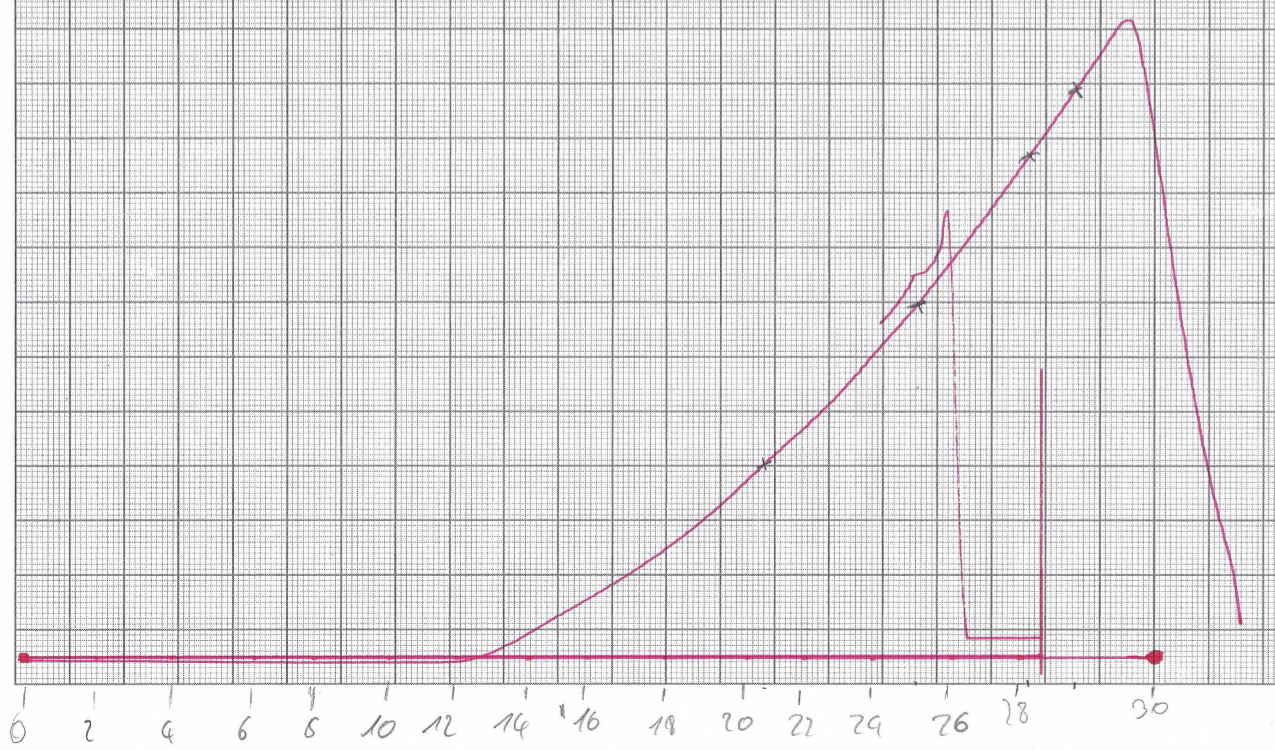
\includegraphics[width=0.8 \textwidth]{./pics/ionisierungsenergie.png}
  \caption{Aufgenommene Kurve für die Bestimmung der Ionisierungsspannung $U\ua{ion}$ bei $T=\SI{104}{\celsius}$. Auf der $x$-Achse ist die Spannung $U\ua{B}$ in $\si{\volt}$ aufgetragen.
          Hingegen gibt die $y$-Achse die Stromstärke $I\ua{A}$ an. Zusätzlich sind die vier Punkte makiert die für die Bestimmung der Ionisierungsspannung verwedent werden.}
  \label{fig: messkurve_ioni}
\end{figure}
Die Bestimmung der Ionisierungsspannung $U\ua{ion}$ erfolgt mit Hilfe einer Ausgleichsrechnung an den Teil der Kurve mit einer positiven Steigung.
Gewählt wurden die in der Tabelle \ref{tab: spannung_abstand_ioni} notierten Punkte.
\begin{table} 
\centering 
\caption{Aus Abbildung \ref{fig: messkurve_ioni} abgelesene Spannung-Abstandspaare.} 
\label{tab: spannung_abstand_ioni} 
\begin{tabular}{S S } 
\toprule  
{$x$-Koordinate in $\si{\centi\meter}$} & {$y$-Koordinate in $\si{\centi\meter}$}  \\ 
\midrule  
 13.9  & 3.5\\ 
16.6  & 7.0\\ 
18.7  & 9.7\\ 
19.6  & 10.9\\ 
\bottomrule 
\end{tabular} 
\end{table}
An diese wurde eine Ausgleichgerade der Form \eqref{eq: gerade} berechnet.
Aus der Regressionsrechnung ergeben sich die Folgenden Parameter
\begin{equation*}
  m=\num{1.296\pm0.004} \qquad b=\SI{-14.52\pm0.07}{\centi\meter}.
\end{equation*}
Das Ergebnis ist zusätzlich in Abbildung \ref{fig: ioni_fit} dargestellt.
\begin{figure}
  \centering
  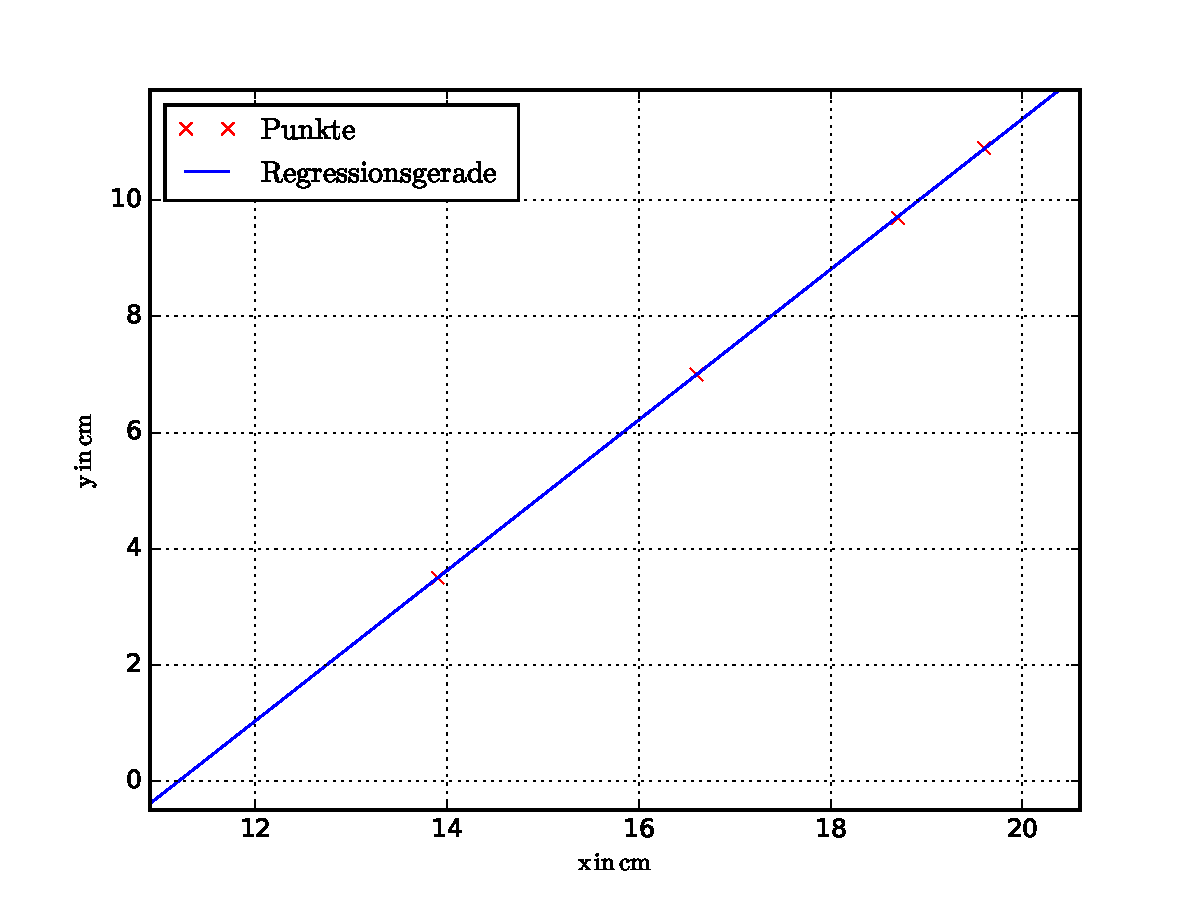
\includegraphics[width=0.8 \textwidth]{../Messdaten/gerade_io_final.pdf}
  \caption{Ausgleichsgerade der aus Abbildung \ref{fig: messkurve_ioni} abgelesenen Punkte.}
  \label{fig: ioni_fit}
\end{figure}
Der Nullpunkt der Ausgleichsgeraden entspricht dann gerade der verschobenen
Ionsiationsspannung:
\begin{equation*}
  U\ua{ion,v}=-\frac{m}{b}=\SI{11.20\pm0.06}{\volt}
\end{equation*}
Die Umrechnung von $\si{\centi\meter}$ zu $\si{\volt}$ erfolgt mit den Ergebnissen aus
Abschnitt \ref{sec: ausgleich}.
Mit Hilfe der zuvor bestimmten Kontakpotentiale $K$ (vgl. \eqref{eq:k_energie_zim} und \eqref{eq:k_frank})
kann $U\ua{ion}$ bestimmt werden. Es ergibt sich für die Ioniersungsspannung:
\begin{equation}
  \label{eq: u_ion}
  U\ua{ion}= U\ua{ion,v}-\ov{K}=\SI{9.74\pm0.14}{\volt} \quad \text{mit} \quad \ov{K}=\SI{1.46\pm0.13}{\volt}.
\end{equation}
Hierbei ist $\ov{K}$ der Mittelwert aus den zuvor bestimmten Kontaktpotentialen.
\FloatBarrier
